\documentclass[aspectratio=43,english]{beamer} %If you want to create Polish presentation, replace 'english' with 'polish' and uncomment 3-th line, i.e., '\usepackage{polski}'
\usepackage[utf8]{inputenc}
\usepackage{polski} %Uncomment for Polish language
\usepackage{babel}
\usepackage{listings} %We want to put listings

\mode<beamer>{ 	%in 'beamer' mode
	\hypersetup{pdfpagemode=FullScreen}		%Enable Full screen mode
	\usetheme{JuanLesPins} 		%Show part title in right footer
	%\usetheme[dark]{AGH}                 		%Use dark background
	%\usetheme[dark,parttitle=leftfooter]{AGH}  	%Use dark background and show part title in left footer
}
\mode<handout>{	%in 'handout' mode
	\hypersetup{pdfpagemode=None}		
	\usepackage{pgfpages}
  	\pgfpagesuselayout{4 on 1}[a4paper,border shrink=5mm,landscape]	%show 4 slides on 1 page
  	\usetheme{boxes}
  	\addheadbox{structure}{\quad\insertpart\hfill\insertsection\hfill\insertsubsection\qquad} 	%content of header
 	\addfootbox{structure}{\quad\insertauthor\hfill\insertframenumber\hfill\insertsubtitle\qquad} 	%content of footer
}

\AtBeginPart{ %At begin part: display its name
	\frame{\partpage}
} 


%%%%%%%%%%% Configuration of the listings package %%%%%%%%%%%%%%%%%%%%%%%%%%
% Source: https://en.wikibooks.org/wiki/LaTeX/Source_Code_Listings#Using_the_listings_package
%%%%%%%%%%%%%%%%%%%%%%%%%%%%%%%%%%%%%%%%%%%%%%%%%%%%%%%%%%%%%%%%%%%%%%%%%%%%
\lstset{ %
  backgroundcolor=\color{white},   % choose the background color
  basicstyle=\footnotesize,        % the size of the fonts that are used for the code
  breakatwhitespace=false,         % sets if automatic breaks should only happen at whitespace
  breaklines=true,                 % sets automatic line breaking
  captionpos=b,                    % sets the caption-position to bottom
  commentstyle=\color{green},      % comment style
  deletekeywords={...},            % if you want to delete keywords from the given language
  escapeinside={\%*}{*)},          % if you want to add LaTeX within your code
  extendedchars=true,              % lets you use non-ASCII characters; for 8-bits encodings only, does not work with UTF-8
  frame=single,	                   % adds a frame around the code
  keepspaces=true,                 % keeps spaces in text, useful for keeping indentation of code (possibly needs columns=flexible)
  keywordstyle=\color{blue},       % keyword style
  morekeywords={*,...},            % if you want to add more keywords to the set
  numbers=left,                    % where to put the line-numbers; possible values are (none, left, right)
  numbersep=5pt,                   % how far the line-numbers are from the code
  numberstyle=\tiny\color{gray},   % the style that is used for the line-numbers
  rulecolor=\color{black},         % if not set, the frame-color may be changed on line-breaks within not-black text (e.g. comments (green here))
  showspaces=false,                % show spaces everywhere adding particular underscores; it overrides 'showstringspaces'
  showstringspaces=false,          % underline spaces within strings only
  showtabs=false,                  % show tabs within strings adding particular underscores
  stepnumber=2,                    % the step between two line-numbers. If it's 1, each line will be numbered
  stringstyle=\color{cyan},        % string literal style
  tabsize=2,	                   % sets default tabsize to 2 spaces
  title=\lstname,                  % show the filename of files included with \lstinputlisting; also try caption instead of title
                                   % needed if you want to use UTF-8 Polish chars
  literate={?}{{\k{a}}}1
           {?}{{\k{A}}}1
           {?}{{\k{e}}}1
           {?}{{\k{E}}}1
           {�}{{\'o}}1
           {�}{{\'O}}1
           {?}{{\'s}}1
           {?}{{\'S}}1
           {?}{{\l{}}}1
           {?}{{\L{}}}1
           {?}{{\.z}}1
           {?}{{\.Z}}1
           {?}{{\'z}}1
           {?}{{\'Z}}1
           {?}{{\'c}}1
           {?}{{\'C}}1
           {?}{{\'n}}1
           {?}{{\'N}}1
}
%%%%%%%%%%%%%%%%%


\title{Metody Obliczeniowe w Nauce i Technice}
\author{Marian Bubak, PhD}
\date{}
\institute[AGH]{
	Institute of Computer Science\\ul. Kawiory 21\\30-055 Krakow\\
	Poland\\
	\url{http://www.icsr.agh.edu.pl/~mownit/}
}


\usepackage{amsmath}
\usepackage{mathtools}
\subtitle{4. Funkcje sklejane - spline functions}
\setcontributors{Mateusz Woś\\Michał Matusiak\\Kamil Doległo}


\begin{document}
  	\maketitle
	%%%%%%%%%%%%%%%%
	\begin{frame}{Outline}
		\tableofcontents
	\end{frame}
	%%%%%%%%%%%%%%%%
	\section{Wprowadzenie}
	\begin{frame}{Wprowadzenie}
    	\textit{Spline} - listwa traserska, krzywik ustawny; wyginany tak, aby
        przechodził przez zadane punkty $\{ x_{i},y_{i} \} \newline \newline$
		\textbf{Teoria elastyczności} - liniał przyjmuje kształt minimalizujący
        energię
        potencjalną $E_{p} \newline$
        $s(x)$ - funkcja $\newline$
        $s''(x)$ - krzywizna, dx - długość łuku $\newline$
        $s,\ s',\ s'' $ - ciągłe w $[x_{i},x_{n}] \newline$
        local curvature: $\frac{f''(x)}{(1+f'(x))^{\frac{5}{2}}}$
        \[
        	\min ! \int_{x_{i}}^{x_{n}}\underbrace{[s''(x)]^{2}dx}_{E_{p}}
            \Rightarrow w_{3}(x)
            \ \ \textrm{na} \ \ [x_{i},x_{i+1}]
        \]
        \[
        	\textrm{"strain energy"} = \int_{a}^{b} 
            \frac{(f''(x))^{2}}{(1+f'(x))^{\frac{5}{2}}}dx
        \]
        
	\end{frame}
    %%%%%%%%%%%%%%%%%%%%%%%%%%%%%%%%%%%%%%%%%%%%%%%%%%
    \begin{frame}{Definicja funkcji sklejanej}
    	\begin{exampleblock}{}
    		Funkcję $s(x) = s(x, \Delta n)$ określona na $[a,b]$ nazywamy funkcją 						sklejaną stopnia m $(m\geq1)$ jeżeli:
            \begin{itemize}
            \item $s(x)$ jest wielomianem stopnia $ \leq m$ na każdym $[x_{i},x_{i+1}]$
            \item $s(x) \in C^{m-1}[a,b]\rightarrow s(x)$ i jej $(m-1)$ pochodnych są ciągłe 				na $[a,b]$
            \end{itemize}
            $\newline$
            $\Delta n$ - podział $[a,b]$ na (n-1) podprzedziałów przez węzły: 
            $a=x_{1}<x_{2}<...<x_{i}<...<x_{n}=b$
    	\end{exampleblock}
		
    \end{frame}
	%%%%%%%%%%%%%%%%%%%%%%%
	\section{Liniowa funkcja sklejana}
	\begin{frame}{Liniowa funkcja sklejana}
    	Interpolacja podziałowa, liniowa: $x\in[x_{i},\ x_{i+1}]:\rightarrow y(x)$
        \[
		y(x)=y_{i}+\frac{y_{i+1}-y_{i}}{x_{i+1}-x_{i}}(x-x_{i})=\underbrace{\frac{x_{i+1}-x}{x_{i+1}-x_{i}}y_{i}}_{\text{$\psi_{i}$}}+\underbrace{\frac{x-x_{i}}{x_{i+1}-x_{i}}y_{i+1}}_{\text{$\psi_{i+1}$}}
		\]
        %%%%%%%%%%%%%%%%%%%%%%%%
        $\newline$
        \textbf{Funkcja kształtu} (shape function)
        \[
        	\psi_{i}(x) = 
            \begin{cases}
            	\frac{x-x_{i}}{x_{i}-x_{i-1}} &x \in [x_{i-1},x_{i}]
            	\\
                \frac{x_{i+1}-x}{x_{i+1}-x_{i}} &x \in [x_{i},x_{i+1}]
             	\\
            	0 &x  \notin [x_{i-1},x_{x+1}]   
            \end{cases}
        \]
        %%%%%%%%%%%%%%%%%%%%%%%%
		\begin{alertblock}{\textbf{Ważne}}
			$\psi_{i}(x_{j})=\sigma_{ij}=f(x)=
            \begin{cases} 0 \ dla \ j\neq i \\1 \ dla \ j=i \end{cases}$
		\end{alertblock}
	\end{frame}
    
    %%%%%%%%%%%%%%%%%%%%%%%%%%%%%%%%%%%%5
    \begin{frame}
        \begin{figure}[h]
			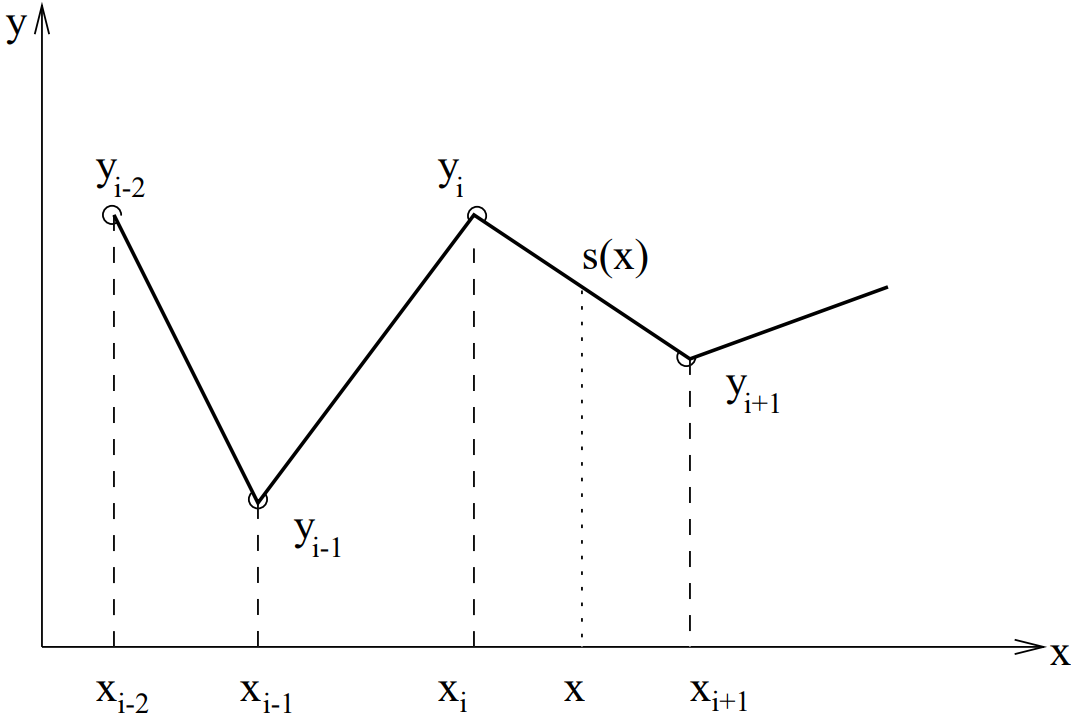
\includegraphics[width=.6\linewidth]{img/4/spline_img_1}
		\end{figure}
		\begin{figure}[h]
			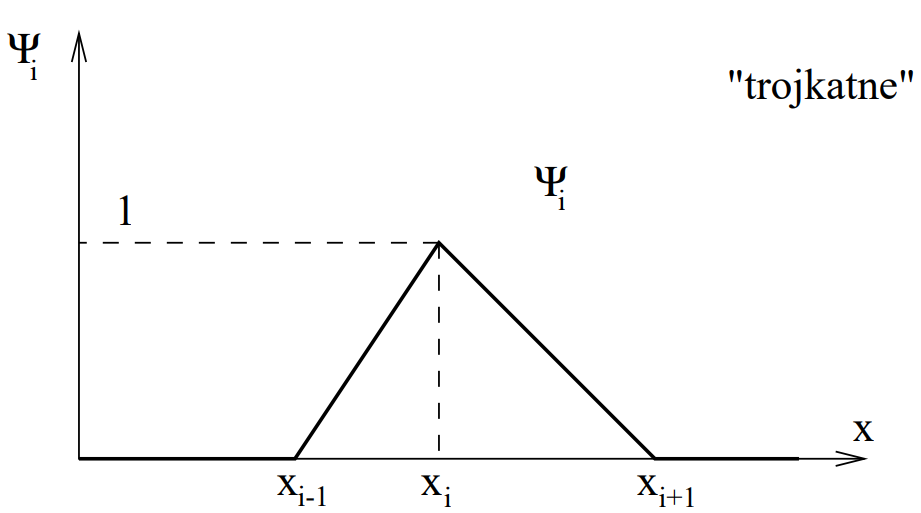
\includegraphics[width=.6\linewidth]{img/4/spline_img_2}
		\end{figure}
    \end{frame}
    
   %%%%%%%%%%%%%%%%%%%%%%%%%%%%%%%5
   \begin{frame}
   		\begin{exampleblock}{}
   			Interpolującą funkcję sklejaną stopnia 1-go można zapisać:
            \[
            	s(x)=\sum_{n=0}^{n}y_{i}\psi_{i}(x)
            \]
            gdzie $\psi_{i}(x), i=0,...,m$ - baza przestrzeni liniowej funkcji sklejanych
            1-go stopnia
   		\end{exampleblock}
        \begin{figure}[h]
			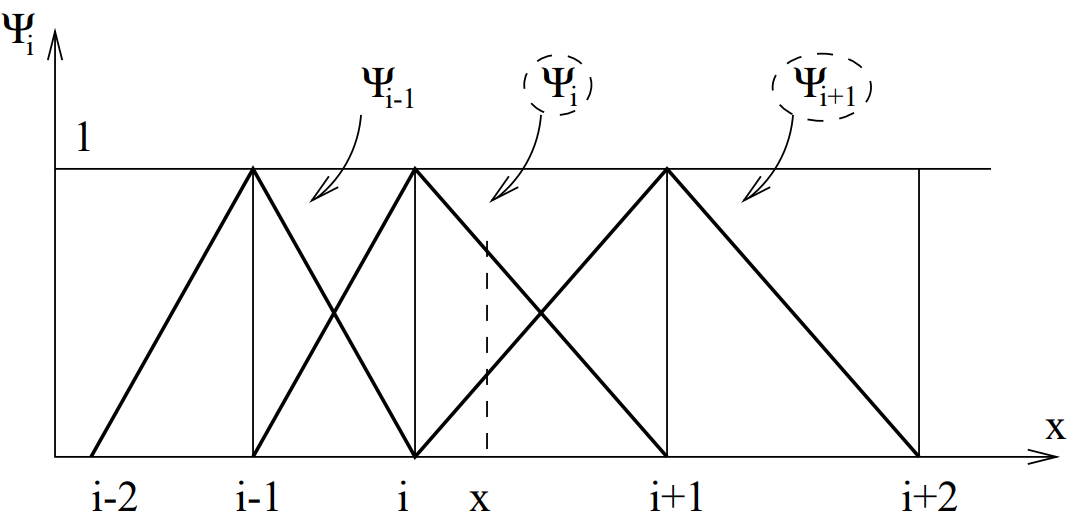
\includegraphics[width=.65\linewidth]{img/4/spline_img_3}
		\end{figure}
   \end{frame}
    
    
    
    
    
    
    
    
    
    
    
    
    
    
    
    
    
    
	%%%%%%%%%%%%%%%%%%%%%%%
	\section{Cubic spline interpolation}
	\begin{frame}{Cubic spline interpolation}
		\begin{block}{}
			\begin{itemize}
				\item $s_{j}$ on $[x_{j},x_{j+1}] \rightarrow$ cubic polinomial:
                $\newline \ \ \ s_{j}(x)=a_{j}+b_{j}(x-x_{j})+c_{j}(x-x_{j})^{2}+
                d_{j}(x-x_{j})^{3}$
                \item $s_{j}x=f(x_{j})(=s_{j-1}(x-j))$
                \item $s_{j}(x_{j+1})=s_{j+1}(x_{j+1})$
                \item $s^{'}_{j}(x_{j+1})=s^{'}_{j+1}(x_{j+1})$
                \item $s^{''}_{j}(x_{j+1})=s^{''}_{j+1}(x_{j+1})$
			\end{itemize}
		\end{block}
        \begin{figure}[h]
			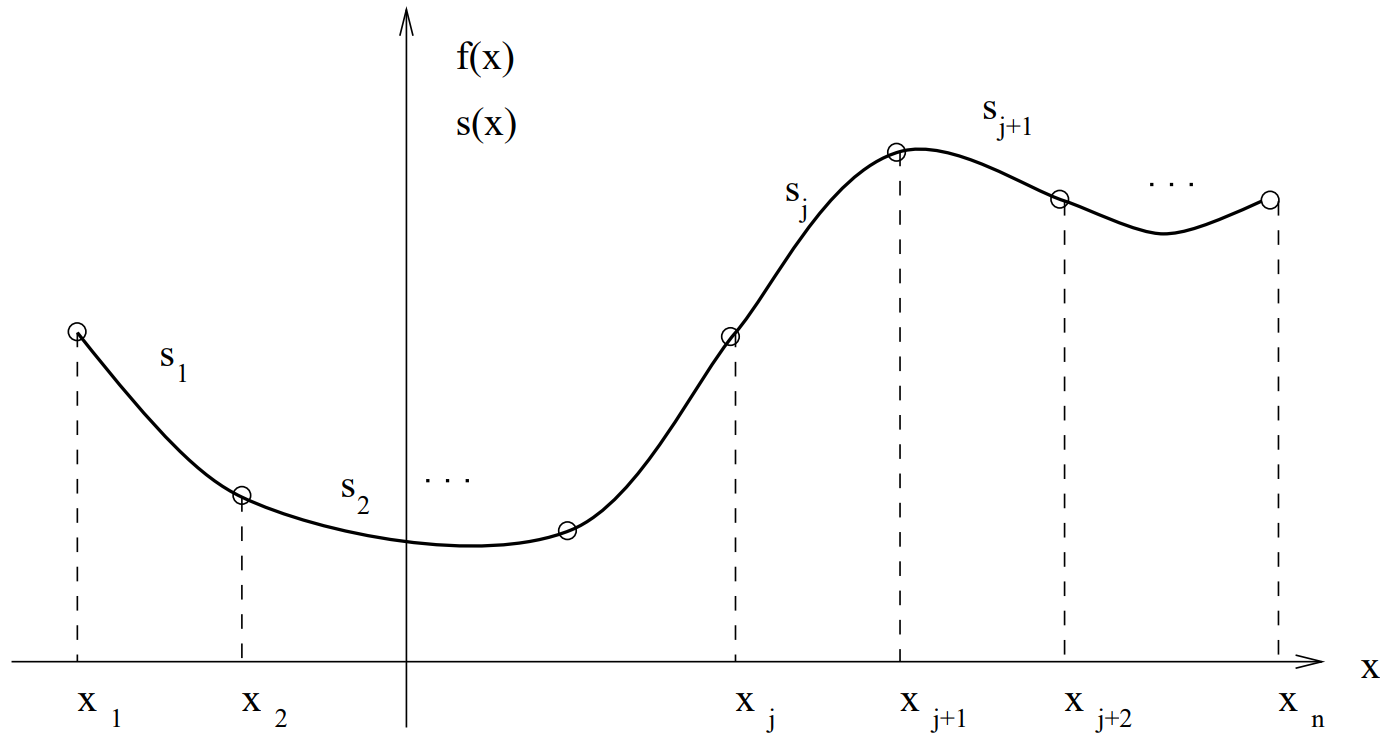
\includegraphics[width=.55\linewidth]{img/4/spline_img_4}
		\end{figure}
	\end{frame}
	%%%%%%%%%%%%%%%%%%%%%%%
\section{Konstrukcja interpolujących sześciennych funkcji sklejanych}
	\begin{frame}{Konstrukcja interpolujących sześciennych funkcji sklejanych}
		Podprzedział $[x_{i},x_{i+1}]$, oznaczmy:
       	\begin{itemize}
       	\item $h_{i}=x_{i+1}-x_{i}$
        \item $w=\frac{x-x_{i}}{h_{i}}$
        \item $\overline{w}=\frac{x_{i+1}-x}{h_{i}}=1-w$
       	\end{itemize}
        $\newline$
        \[
        	x \nearrow \ od \ x_{i} \ do \ x_{i+1}: \ \ \ w:\nearrow \ 0 \rightarrow 1, 
            \ \overline{w}:\searrow \ 1 \rightarrow 0
        \]
       
	\end{frame}
    %%%%%%%%%%%%%%%%%%%%%%%%%%%%%%%5
    \begin{frame}
    	 Niech dla $[x_{i},x_{i+1}]$ sześcienna funkcja sklejana ma postać:
        \[
        	s(x)= \underbrace{w\cdot y_{i+1}+\overline{w} \cdot y_{i}}_{\text{$(*)$}}
            + \underbrace{h^{2}_{i}[(w^{3}-w)\sigma_{i+1}+
            (\overline{w}^{3}-\overline{w})\sigma_{i}]}_{\text{$(**)$}}
        \]
        gdzie:
        $\newline(*)$ - człony standardowej interpolacji liniowej
        $\newline(**)$ - korekta sześcienna - dodatkowe wygładzanie funkcji
        $\newline \sigma_{i}, \sigma_{i+1}$ - pewne stałe, do wyznaczenia
        $\newline$
        \begin{itemize}
        	\item Człony korekcyjne znikają na końcach przedziału $[x_{i},x_{i+1}]$
            \item $s(x_{i})=y_{i}; \ \ s(x_{i+1})=y_{i+1} \newline$
            	niezależnie od wyboru $\sigma_{i} \Rightarrow s(x)$ interpoluje dane:
                $\{ x_{i},y_{i} \}$
        \end{itemize}
    \end{frame}
    %%%%%%%%%%%%%%%%%%%%%%%
    \begin{frame}
		Różniczkujemy $s(x)$ korzystając z:
        \[
        	w'=\frac{dw}{dx}=\frac{1}{h_{i}}\ ;\ \overline{w}'=-\frac{1}{h_{i}}
        \]
        \begin{itemize}
        	\item $s'(x)=\frac{y_{i+1}-y_{i}}{h_{i}}+h_{i}[(3w^{2}-1)\sigma_{i+1}-
            			(3\overline{w}^{2}-1)\sigma_{i}],  \  \ \textbf{(*)}$
            \item $s''(x)=6w\sigma_{i+1}+6\overline{w}\sigma_{i}  \ \ 
            	\Rightarrow 
            	\framebox{$\sigma_{i}=\frac{1}{6}s''(x_{i})$}$ sens stałych $\sigma_{i}$
            \item $s'''(x)=\frac{6}{h_{i}}(\sigma_{i+1}-\sigma_{i})=
            	const \newline$
              	 - zgodnie z tym, że $s(x)$ jest lokalnie sześcienna 
        \end{itemize}
        \begin{block}{}
        	$\sigma_{i} \ $- określa wartości $s''(x)$ w węzłach (punktach granicznych)
            $\newline$
            $\hspace*{0.5cm}$ - automatycznie zapewnia ciągłość 2-gich pochodnych
        \end{block}
    \end{frame}
    %%%%%%%%%%%%%%%%%%%%%%%
    \begin{frame}
    	Wartości $\sigma_{i}$ - z warunku ciągłości $s'(x)$ w węzłach: 
        $\Delta_{i}=\frac{y_{i+1}-y_{i}}{h_{i}} \newline \newline$
        Z $\textbf{(*)}$: 
        $
        \begin{cases}
            	s_{+}'(x_{i})  &=\ \Delta_{i}-h_{i}(\sigma_{i+1}+2\sigma_{i})
            	\\
                s_{-}'(x_{i+1}) &=\ \Delta_{i}+h_{i}(2\sigma_{i+1}+\sigma_{i}) 
        \end{cases}
        $
        \begin{block}{}
        	\centering Warunek ciągłości: $s_{-}'(x_{i}) = s_{+}'(x_{i})$
        \end{block}
        $s_{-}'(x_{i})$ wyznaczane z $\textbf{(*)}$ dla $[x_{i-1},x_{i}]$:
        \[
        	\framebox{$\Delta_{i-1}+h_{i-1}(2\sigma_{i}+\sigma_{i-1})=
            \Delta_{i}-h_{i}(\sigma_{i+1}+2\sigma_{i})$}
        \]
        otrzymujemy układ (n-2) równań liniowych  (dla punktów pośrednich):
        \[
        	h_{i-1}\sigma_{i-1}+2(h_{i-1}+h_{i})\sigma_{i}+h_{i}\sigma_{i+1}=
            \Delta_{i}-\Delta_{i-1}, \ \ i=2, 3, . . . , n-1
        \]
        ale ponieważ mamy n niewiadomych $\sigma_{i}$ konieczne jest
        określanie dwóch dodatkowych warunków.
    \end{frame}
    %%%%%%%%%%%%%%%%%%%%%%%
    \begin{frame}
		$\newline$
    	Istnieje wiele sposobów określania dodatkowych warunków.
       \begin{enumerate}
       \item  \[
		\begin{rcases*}
			C_{1}(x) - \textrm{f. sześcienna przez pierwsze 4 punkty}\\
			C_{n}(x) - \textrm{f. sześcienna przez ostatnie 4 punkty}
		\end{rcases*} \rightarrow
		\]	
       \end{enumerate}	
       \[
       		\framebox{$s'''(x_{1})=C^{'''}_{1}\ \ \ s'''(x_{n})=C^{'''}_{n}$}
       \]
        Stałe $C^{'''}_{1}$ i $C^{'''}_{n}$ mogą być określone bez znajomości 
        $C_{1}(x)$ i $C_{n}(x)$:
        \[
        	\Delta_{i}\ =\ \frac{y_{i+1}-y_{i}}
            {x_{i+1}-x_{i}}\ ;\ \textrm{przybliża 1-szą pochodną}
        \]
        \[
        	\Delta_{i}^{(2)}=\frac{\Delta_{i+1}-\Delta_{i}}
            {x_{i+2}-x_{i}}\ ;\ 2\Delta_{i}^{(2)}\approx f^{''}
        \]
        \[
        	\Delta_{i}^{(3)}\ =\ \frac{\Delta_{i+1}^{(2)}-\Delta_{i}^{(2)}}
            {x_{i+3}-x_{i}}\ ;\ 6\Delta_{i}^{(3)}\approx f^{'''}
        \]
    \end{frame}
    %%%%%%%%%%%%%%%%%%%%%%
    \begin{frame}
    	i ogólnie dla:
        \begin{flushright}
        	$f[x_{0}]\equiv f(x_{0}) \linebreak \linebreak$
            $f[x_{0},\ x_{1}]\equiv\frac{f[x_{1}]-f[x_{0}]}{x_{1}-
            x_{0}}=\frac{f(x_{1})-f(x_{0})}{x_{1}-x_{0}} 
            \linebreak \linebreak$
            $f[x_{0},\ x_{1},\ x_{2}]\equiv\frac{f[x_{1},x_{2}]-f[x_{0},x_{1}]}
            {x_{2}-x_{0}} \linebreak $
            $\ldots \ldots \linebreak$
            $f[x_{0},\ x_{1},\ .\ .\ .\ ,\ x_{k}]\equiv\frac{f[x_{1},\ldots,x_{k}]-f[x_{0},\ldots,x_{k-1}]}{x_{k}-x_{0}}$
        \end{flushright}
        mamy związek między ilorazami różnicowymi a pochodnymi:
        \begin{exampleblock}{}
        	$
            	\centering f[x_{0}, ... \ , x_{n}]=\frac{f^{(n)}(\eta)}
                {n!}, \ \ \ \eta \in [x_{0},... \ , x_{n}]
                \ \ \ (\eta \textrm{- pewien punkt})
            $
        \end{exampleblock}
        \begin{block}{Zadanie}
        	Sprawdzić
        \end{block}
        
    \end{frame}
    %%%%%%%%%%%%%%
    \begin{frame}
    	zatem:
        \begin{align*}
        	s'''(x_{1})&=c_{1}'''(x_{1}) \Rightarrow
            \frac{6}{h_{1}}(\sigma_{2}-\sigma_{1})=6\Delta_{1}^{(3)}
            &|\cdot h_{1}^{2}
            \\
            s'''(x_{n})&=c_{n}'''(x_{1}) \Rightarrow
            \frac{6}{h_{n-1}}(\sigma_{n}-\sigma_{n-1})=6\Delta_{n-3}^{(3)}
            &|\cdot h_{n-1}^{2}
        \end{align*}
        po przekształceniu: (cel = symetria)
        $\newline \newline
        \begin{cases}
        	-h_{1}\sigma_{1}+h_{1}\sigma_{2}=h_{1}^{2}\Delta_{1}^{(3)}
            \\
		h_{n-1}\sigma_{n-1}-h_{n-1}\sigma_{n}=-h_{n-1}^{2}\Delta_{n-3}^{(3)}
        \end{cases}
        $
    \end{frame}
    %%%%%%%%%%%%%%%%%%
    \begin{frame}
    	mamy:
        \[
        \begin{bmatrix}
    -h_{1} & h_{1} & 0 & 0  & 0 \\
    h_{1} & 2(h_{i}+h_{2}) & h_{2} & 0  & 0 \\
    0 & h_{2} & 2(h_{2}+h_{3}) & h_{3} & 0 \\
    \vdots & \vdots & \vdots & \vdots & \vdots \\
    0 & 0 & h_{n-2} & 2(h_{n-2}+h_{n-1}) & h_{n-1} \\
    0 & 0 & 0 & h_{n-1}  & -h_{n-1}
		\end{bmatrix}
        \begin{bmatrix}
        	\sigma_{1} \\
            \sigma_{2} \\
            \sigma_{3} \\
            \vdots \\
            \sigma_{n-1} \\
            \sigma_{n}
        \end{bmatrix}
       	=
        \]
        \[	=
        	\begin{bmatrix}
        		h_{1}^{2}\Delta^{(3)}_{i} \\
                \Delta_{2} - \Delta_{1} \\
                \Delta_{3} - \Delta_{2} \\
                \vdots \\ 
                \Delta_{n-1} - \Delta_{n-2} \\
                \Delta_{n} - \Delta_{n-1}
        	\end{bmatrix}
        \]
    \end{frame}
    %%%%%%%%%%%%%%%%%%
    \begin{frame}{Inne ważne możliwości określania warunków}
    	\begin{enumerate}
        \setcounter{enumi}{1}
    		\item natural cubic spline: $s''(x_{1})=s''(x_{n})=0$ (free boundary)
            \item complete spline: $s'(x_{1})=y'_{1}, \ \ s'(x_{n})=y'_{n}$
            (clamped boundary)
            \item $s''(x_{1})=y''_{1}; \ \ s^{n}(x_{n})=y''_{n}$
            \item $s'''(x)$ ciągła w $x_{2}$ oraz $x_{n-1}$ (not-a-knot condition)
            \item interpolowanie spline'ami funkcji periodycznych
    	\end{enumerate}
    \end{frame}
    %%%%%%%%%%%%%%%%%%%%
    \begin{frame}
    	\begin{block}{Zadanie 1}
        	Dla obliczeń - zwłaszcza wielokrotnego określania wartości s(x) 
            korzystna jest postać:
            \[
            	s(x)=y_{i}+b_{i}\cdot(x-x_{i})+c_{i}
                \cdot(x-x_{i})^{2}+d_{i}\cdot(x-x_{i})^{3}
                \ \ dla \ x\in[x_{i},\ x_{i+1}]
            \]
            $b_{i}, c_{i}, d_{i}$ - określone dla każdego przedziału:
            $b_{i}=\frac{y_{i+1}-y_{i}}{h_{i}}-h_{i}\cdot (\sigma_{i+1}
            +2\sigma_{i})\newline$
            $c_{i}=3\cdot \sigma_{i}\newline$
            $d_{i}=\frac{\sigma_{i+1}-\sigma_{i}}{h_{i}}\newline$
            Sprawdzić.
        \end{block}
        \begin{block}{Zadanie 2}
    		Układ równań dla 
            $s_{i}(x)=a_{i}+b_{i}(x-x_{i})+c_{i}(x-x_{i})^{2}+d_{i}
            (x-x_{i})^{3}$
            $\newline$
            (obliczenie $\rightarrow$ Horner) $\rightarrow$ 
            podejście "wprost"
    	\end{block}
    \end{frame}
    %%%%%%%%%%%%%%%%%%%%
    \begin{frame}{Błąd interpolacji funkcji sklejanych}
    	gdy:
        \begin{itemize}
        \item $a=x_{1}, x_{2}, . . . , x_{n}=b$
        \item $f\in C^{4}[a,\ b] , \ \ \ \ \max_{x\in[a,b]}|f^{(4)}
        (x)|\leq M$
        \item $s'(x_{1})=f'(x_{1}), \ \ \ s'(x_{n})=f'(x_{n})$
        \end{itemize}
        to:
        \[
        	\max_{x\in[a,b]}|f(x)-s(x)|\leq \frac{5}{384} \cdot
            M \cdot \max_{1 \leq i \leq n-1}(x_{i+1}-x_{i})^{4}
        \]
    \end{frame}
    
    
    
    
    
    
    
    
    
    
    
    
    
    
    
    
    
    
    
    
    
    

    
    
    
    
    
    
    
    
    
    
    
    
    
    
    
    
    
    
    
	%%%%%%%%%%%%%%%%%%%%%%%
	\section{Zalety funkcji sklejanych}
\begin{frame}{Zalety}
	\begin{itemize}
	\item dokładniejsza, bezpieczniejsza interpolacja - patrz rysunek!
    \begin{figure}[h]
			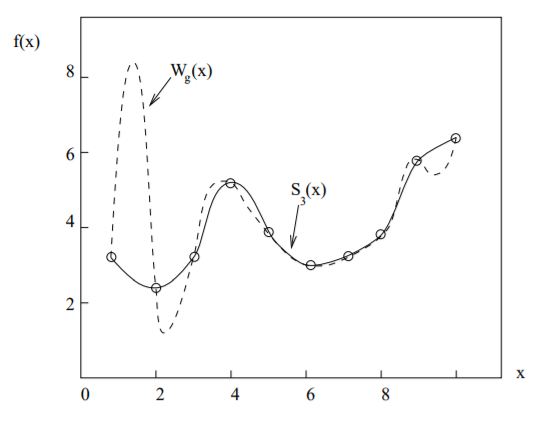
\includegraphics[width=.75\linewidth]{img/4/spline_img_5}
		\end{figure}
	\end{itemize}
\end{frame}
%%%%%%%%%%%%%%%%
\begin{frame}{Zalety c.d.}
	\begin{itemize}
		\item wartości $s_{3}(x)$ łatwe do wyznaczania
    	\item w praktyce - $s_{3}$ wystarczające
    	\item przydatne dla węzłów równoodległych
    	\item można używać dla określenia $\Rightarrow \frac{d^{(n)}}	
        	{dx^(n)}f(x)$
    		i $\int f(x)dx$ 
	\end{itemize}
	\begin{block}{Zadanie 1}
        	$s'(x), \ s''(x)$
    \end{block}
    \begin{block}{Zadanie 2}
        	$\int^{x_{n}}_{x_{1}}s(x)dx$
    \end{block}
\end{frame}
%%%%%%%%%%%%%%%%
\begin{frame}{Zastosowania}
	\begin{itemize}
		\item do wygładzania powierzchni:
        	\begin{itemize}
        		\item siatka porotokątna $(x_{i},y_{i})$, $i=1,2,...,m$; 
                	$j=0,1,...,n$
                \item funkcje sklejane na siatce, np.: 
                \[
                	\framebox{$s(x,y)=\sum_{i=0}^{m}\sum_{j=0}^{n}f(x_{i},
                    \ y_{i})\psi_{i}(x)\psi_{j}(y)$}
                \]
                %% dead link
        	\end{itemize}
	\end{itemize}
\end{frame}
%%%%changed encoding of file, utf-8 -> utf-8(without BOM)








	%%%%%%%%%%%%%%%%%%%%%%%
	\section{B-splines - basic splines}
\begin{frame}
	$B_{j,k}(x)$ - B-spline rzędu k:
    \begin{itemize}
    \item  $B_{j,1}=
        \begin{cases}
            	1  &,\ x_{j} \leq x \leq x_{j+1}
            	\\
                0 &,\ \textrm{poza przedziałem}
        \end{cases}
        $
        \item wyższe rzędy $(k>1)$ - rekurencyjnie:
        \[
        	B_{j,k}=\frac{x-x_{j}}{x_{j+k-1}-x_{j}}B_{j,k-1}(x)+\frac{x_{j+k}-x}
            {x_{j+k}-x_{j+1}}B_{j+1,k-1}(x)
        \]
        \item $B_{j,k}(x)=\{>0, x\in[x_{j},\ x_{j+k}]=0\} \ \ x 
        \textrm{- poza przedziałem}$
        \item w przedziale $[x_{j},\ x_{j+1}]$ tylko $k$: $B_{j-k+1,k}(x)\ldots
        B_{j,k}(x)\neq 0$
		\item normalizacja: $\sum_{j}B_{j,k}(x)=\sum_{j=l+1-k}^{l}B_{j,k}(x)=1$ 
        \newline dla $x_{l}\leq x\leq x_{l+1}$
\end{itemize}
\end{frame}
%%%%%%%%%%%%%%%%%%%%%%%%
\begin{frame}
	\begin{exampleblock}{Reprezentacja funkcji sklejanej stopnia k-1}
		\centering $S(x)=\sum_{j}a_{j}B_{j,k}(x)$
	\end{exampleblock}
    $k=4 \rightarrow$ cubic B-splines: $B_{j,4}(x)=b_{j}(x)$
    $
    \begin{rcases*}
			x \in [a,b]\\
			m - \textrm{B-splines} \ \  b_{j}(x)
		\end{rcases*}\Rightarrow \textrm{odległość między sąsiednimi węzłami}
    $
    $\newline \newline \newline$
    $d = \frac{b-a}{m-3} \newline$
    $(m+4) \textrm{węzły} \ \newline$
    $x_{4}=a \newline$
    $x_{m+1}=b \newline$
    $x_{j}=a+(j-4)d$
\end{frame}
%%%%%%%%%%%%%%%%%%%%%%%%
\begin{frame}
	\begin{figure}[h]
			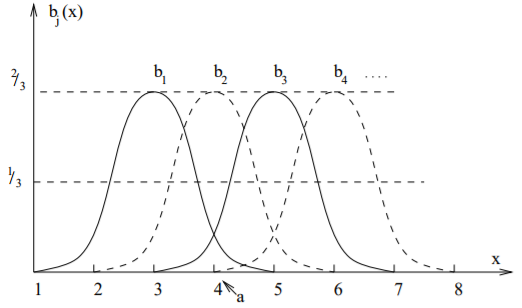
\includegraphics[width=.57\linewidth]{img/4/spline_img_6}
	\end{figure}
    \begin{block}{Zadanie}
    	$B_{j,k}$ dla równoodległych węzłów
    \end{block}
    \[	b_{j}(x)=
    	\begin{cases}
    		\frac{1}{6}z^{3} &,z=\frac{x-x{j}}{d} \ \ x \in [x_{j},x_{j+1}] \\
            \frac{1}{6}[1+3(1+z(1-z))z] &,z=\frac{x-x_{j+1}}{d} \ x 
            \in [x_{j+1},x_{j+2}]\\
            \frac{1}{6}[1+3(1+z(1-z))(1-z)] &,z=\frac{x-x_{j+2}}{d} \ x 
            \in [x_{j+2},x_{j+3}] \\
            \frac{1}{6}(1-z)^{3} &,z=\frac{x-x_{j+3}}{d} \ x 
            \in [x_{j+3},x_{j+4}] \\
            0 \ &, x \notin [x_{j},x_{j+4}]
    	\end{cases}
    \]
\end{frame}
%%%%%%%%%%%%%%%%%%%%%%%%
\begin{frame}{Zastosowanie}
	\begin{itemize}
	\item ogólne zastosowanie B-spilne'ów - 
    	$\newline$encyklopedia matematyczna $\newline$
    		(autor: Copenhagen University Astronomical Observatory)
    \item w grafice komputerowej %deadlink
	\end{itemize}
\end{frame}
%%%%%%%%%%%%%%%%%%%%%%%
\begin{frame}
	\begin{figure}[h]
			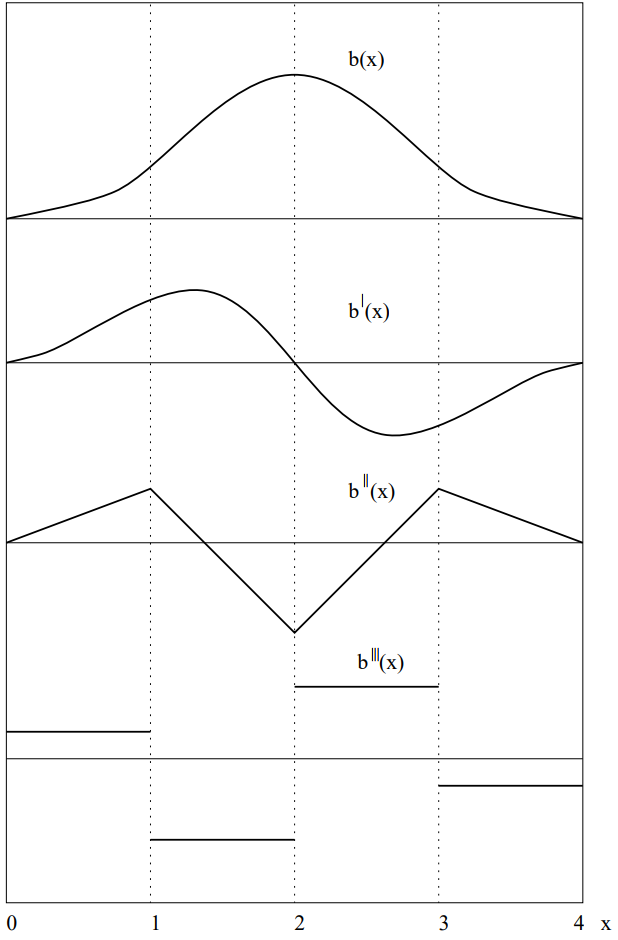
\includegraphics[width=.52\linewidth]{img/4/spline_img_7}
	\end{figure}
\end{frame}





	%%%%%%%%%%%%%%%%%%%%%%%
	\section{Literatura}
\begin{frame}{Literatura}
	\begin{thebibliography}{9}
   		\setbeamertemplate{bibliography item}[article]
            \bibitem{schoenberg} I. J. Schoenberg
            \newblock Contributions to the problem of approximation of equidistant data by analytic functions
            \newblock  Quart. Appl. Math., vol. 4, 1946
		\setbeamertemplate{bibliography item}[book]
            \bibitem{boor} Carl de Boor 
            \newblock A practical guide to splines
            \newblock Springer, 1978
		\setbeamertemplate{bibliography item}[book]
            \bibitem{schultz} M. M. Schultz 
            \newblock Spline analysis 
            \newblock Prentice Hall, 1996
     	\setbeamertemplate{bibliography item}[book]
                 \bibitem{stoer} J. Stoer, R.Bulitsch 
                 \newblock Wstęp do analizy numerycznej 
                 \newblock Państwowe Wydawnictwo Naukowe, 1987
    \end{thebibliography}
\end{frame}
	%%%%%%%%%%%%%%%%%%%%%%%
\end{document}
